\documentclass[tikz,border=5pt]{standalone}
\usepackage[T1]{fontenc}
\usepackage{lmodern,amsmath,amssymb}
\usetikzlibrary{arrows.meta,calc,positioning,fit,backgrounds,shapes.geometric,matrix,decorations.pathreplacing,patterns}
\definecolor{ink}{gray}{0.08}
\definecolor{wash}{gray}{0.965}
\definecolor{soft}{gray}{0.45}
\tikzset{box/.style={draw=ink,line width=.65pt,fill=white,align=center,inner sep=4pt,outer sep=0pt,font=\small},flow/.style={draw=ink,line width=.65pt,-{Latex[length=1.8mm,width=1.3mm]},rounded corners=2pt},annotation/.style={font=\scriptsize,text=soft,align=center},groupbox/.style={draw=soft,dashed,line width=.45pt,fill=wash}}
\begin{document}
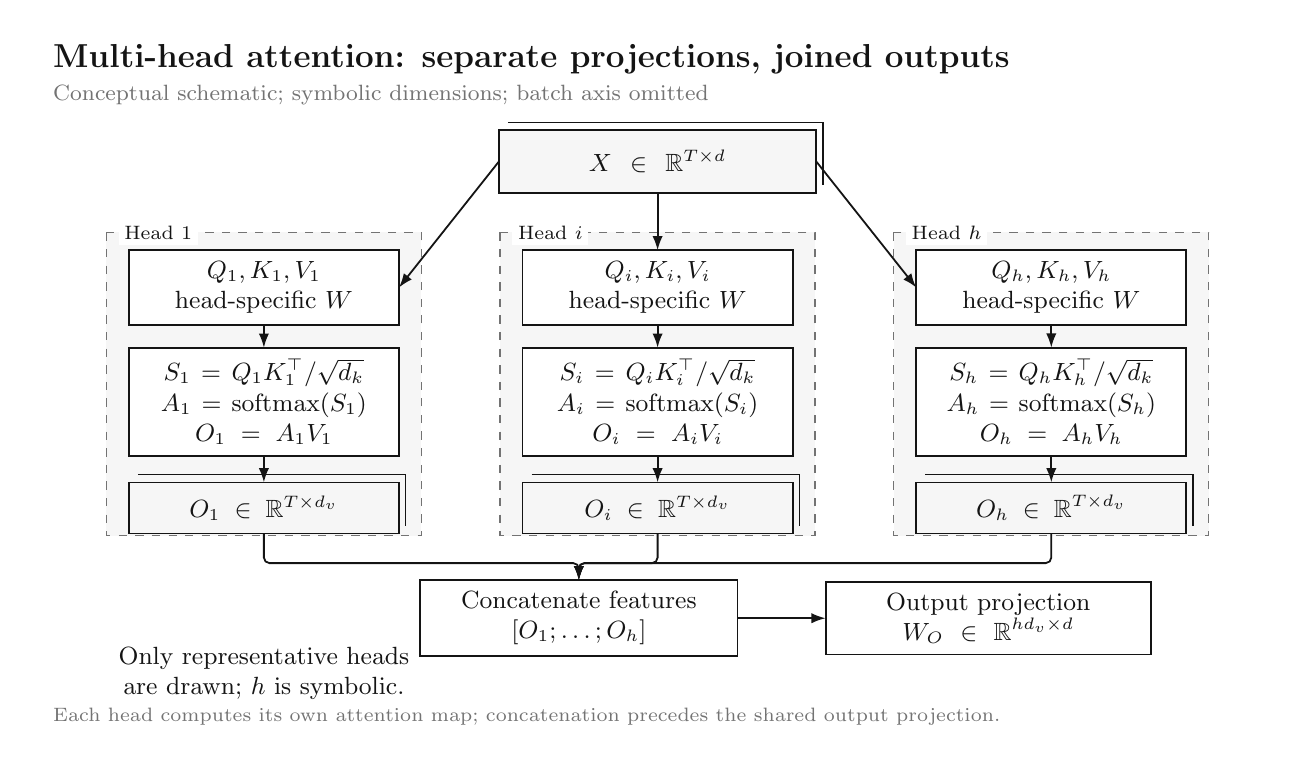
\begin{tikzpicture}[x=1cm,y=-1cm,font=\rmfamily,text=ink]

\path[use as bounding box] (0,0) rectangle (16,9);
\node[anchor=west,font=\large\bfseries] at (.2,.4) {Multi-head attention: separate projections, joined outputs};
\node[anchor=west,font=\footnotesize,text=soft] at (.2,.85) {Conceptual schematic; symbolic dimensions; batch axis omitted};
\begin{pgfonlayer}{background}
\draw[groupbox] (1.0,2.6) rectangle (5.0,6.45);
\node[anchor=west,font=\scriptsize,fill=white,inner sep=2pt] at (1.15,2.6) {Head $1$};
\draw[groupbox] (6.0,2.6) rectangle (10.0,6.45);
\node[anchor=west,font=\scriptsize,fill=white,inner sep=2pt] at (6.15,2.6) {Head $i$};
\draw[groupbox] (11.0,2.6) rectangle (15.0,6.45);
\node[anchor=west,font=\scriptsize,fill=white,inner sep=2pt] at (11.15,2.6) {Head $h$};
\end{pgfonlayer}
\node[box,fill=wash,minimum width=4cm,minimum height=0.8cm,text width=3.75cm] (x) at (8,1.7) {$X\in\mathbb{R}^{T\times d}$};
\draw[ink,line width=.4pt] (6.1,1.1999999999999997) -- (10.1,1.1999999999999997) -- (10.1,2.0);
\node[box,minimum width=3.4cm,minimum height=0.9cm,text width=3.15cm] (proja) at (3,3.3) {$Q_{1},K_{1},V_{1}$\\head-specific $W$};
\node[box,minimum width=3.4cm,minimum height=1.15cm,text width=3.15cm] (attna) at (3,4.75) {$S_{1}=Q_{1}K_{1}^{\top}/\sqrt{d_k}$\\$A_{1}=\operatorname{softmax}(S_{1})$\\$O_{1}=A_{1}V_{1}$};
\node[box,fill=wash,minimum width=3.4cm,minimum height=0.65cm,text width=3.15cm] (oa) at (3,6.1) {$O_{1}\in\mathbb{R}^{T\times d_v}$};
\draw[ink,line width=.4pt] (1.4000000000000001,5.675) -- (4.8,5.675) -- (4.8,6.325);
\node[box,minimum width=3.4cm,minimum height=0.9cm,text width=3.15cm] (projb) at (8,3.3) {$Q_{i},K_{i},V_{i}$\\head-specific $W$};
\node[box,minimum width=3.4cm,minimum height=1.15cm,text width=3.15cm] (attnb) at (8,4.75) {$S_{i}=Q_{i}K_{i}^{\top}/\sqrt{d_k}$\\$A_{i}=\operatorname{softmax}(S_{i})$\\$O_{i}=A_{i}V_{i}$};
\node[box,fill=wash,minimum width=3.4cm,minimum height=0.65cm,text width=3.15cm] (ob) at (8,6.1) {$O_{i}\in\mathbb{R}^{T\times d_v}$};
\draw[ink,line width=.4pt] (6.3999999999999995,5.675) -- (9.799999999999999,5.675) -- (9.799999999999999,6.325);
\node[box,minimum width=3.4cm,minimum height=0.9cm,text width=3.15cm] (projc) at (13,3.3) {$Q_{h},K_{h},V_{h}$\\head-specific $W$};
\node[box,minimum width=3.4cm,minimum height=1.15cm,text width=3.15cm] (attnc) at (13,4.75) {$S_{h}=Q_{h}K_{h}^{\top}/\sqrt{d_k}$\\$A_{h}=\operatorname{softmax}(S_{h})$\\$O_{h}=A_{h}V_{h}$};
\node[box,fill=wash,minimum width=3.4cm,minimum height=0.65cm,text width=3.15cm] (oc) at (13,6.1) {$O_{h}\in\mathbb{R}^{T\times d_v}$};
\draw[ink,line width=.4pt] (11.4,5.675) -- (14.799999999999999,5.675) -- (14.799999999999999,6.325);
\node[box,minimum width=4cm,minimum height=0.9cm,text width=3.75cm] (cat) at (7,7.5) {Concatenate features\\$[O_1;\ldots;O_h]$};
\node[box,minimum width=4.1cm,minimum height=0.9cm,text width=3.8499999999999996cm] (wo) at (12.2,7.5) {Output projection\\$W_O\in\mathbb{R}^{h d_v\times d}$};
\node[align=center,inner sep=0pt,outer sep=0pt,font=\small,minimum width=5.2cm,minimum height=0.4cm,text width=4.95cm] (note12) at (3.0,8.2) {Only representative heads are drawn; $h$ is symbolic.};
\begin{pgfonlayer}{background}
\draw[flow] (x.west) -- (proja.east);
\draw[flow] (proja.south) -- (attna.north);
\draw[flow] (attna.south) -- (oa.north);
\draw[flow] (x.south) -- (projb.north);
\draw[flow] (projb.south) -- (attnb.north);
\draw[flow] (attnb.south) -- (ob.north);
\draw[flow] (x.east) -- (projc.west);
\draw[flow] (projc.south) -- (attnc.north);
\draw[flow] (attnc.south) -- (oc.north);
\draw[flow] (oa.south) -- (3,6.8) -- (7,6.8) -- (cat.north);
\draw[flow] (ob.south) -- (8,6.8) -- (7,6.8) -- (cat.north);
\draw[flow] (oc.south) -- (13,6.8) -- (7,6.8) -- (cat.north);
\draw[flow] (cat.east) -- (wo.west);
\end{pgfonlayer}
\node[anchor=west,align=left,font=\scriptsize,text=soft,text width=15.6cm] at (.2,8.75) {Each head computes its own attention map; concatenation precedes the shared output projection.};
\end{tikzpicture}
\end{document}
